\chapter{\protect Methods}
\label{methods}

\section{Laboratory Astrophysics}
To study the chemical reactivities in astrophysical environments (surface of Charon during winter time) experimentally,
we conduct our experiments in Interstellar photoprocessing system (IPS) \cite{chen2013vacuum},
an ultrahigh vacuum chamber with base pressure $3 \times 10^{-10}$ torr. By ideal gas law, the pressure corresponded to a density of 2$\times$10$^8$ molecules cm$^{-3}$, which is similar to dense cloud interiors. We would like to particularly simulate the surface of Charon. The surface pressure of Charon is however not specific to high VU cross-section gases are not well defined yet, which will be in a future report by New horizons team, while all known species in Pluto's atmosphere to be below 0.3 nano bars (2.25 $\times$ 10$^(-7)$ torr) \cite{stern2017new}.
The system will be introduced in detail in section \ref{sec:IPS_system}.
To simulate the irradiation in interstellar environments,
we use a micro-wave discharge hydrogen lamp (MDHL) and monochromatic extreme-ultraviolet irradiation (EUV) 30.4 nm (40.8 eV)to irradiate our ice mixtures,
and these will be introduced in section \ref{sec:Vacuum_UV_source} and \ref{sec:Extreme_EUV_source} respectively.
The experimental protocols will be elaborated in section \ref{sec:Experimental_Protocol}.
For some non-physic background readers, basic theories of Infrared spectroscopy and basic chemical kinetics used in data analysis are included in section \ref{sec:spectroscopy} and \ref{sec:Reaction_Rate_Laws} respectively.\\

\subsection{Experimental simulations by IPS system}
\label{sec:IPS_system}

We conduct our astrophysical simulations in Interstellar Photo Processing System (IPS) (figure \ref{fig:system}). IPS consists in three systems: the main chamber, where our experiments take places; the detection system, where we collect our data; and a gasline system, where we prepare our samples.

\begin{figure}
\centering
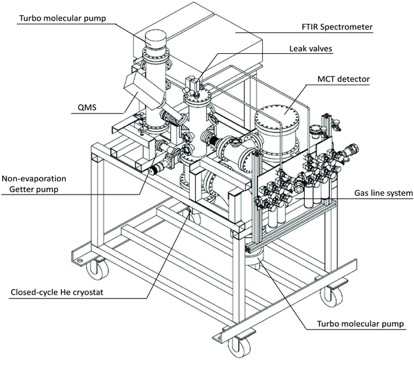
\includegraphics[width=\textwidth]{figures/chapter2/system.jpg}
\caption{The schematic diagram of IPS system, mechanical pumps are not shown for clarity. (Quoted from Chen et al. 2014)}
\label{fig:system}
\end{figure}

The main system consists of an ultrahigh vacuum chamber equips with a closed-cycle helium cryostat (CTI-M350). It is pumped by a turbo molecular pump, which is backed up by a scroll pump, and a non –evaporation getter pump. The getter pump, with a larger surface area, is a powerful tool to adsorb residue gases (H$_2$, CO and N$_2$) inside the main chamber, which can obtain a better base pressure. After baking, the base pressure of our main chamber can reach $1 \times 10^{-10}$ torr at 15 K, monitored by a Granville-Phillips 370 Stabil-Ion gauge. This pressure can be used to simulate the dense cloud interior environments and star forming region. The substrate we have chosen is KBr, which is transparent to infra-red photons with 700 to 4000 $cm^{-1}$. It is mounted by substrate holder(oxygen-free copper), on the second stage of cold finger, which is on the tip of cryostat. A silicon diode and a heater are placed onto the cold finger, and another silicon diode is placed on the substrate holder. They are connected to a temperature controller and PID (proportional–integral–derivative controller) system to achieve a warmup rate of 1K/min with an accuracy of 0.1 K.

The detection system consists of a mid-infrared Fourier transform spectrometer (mid-FTIR) (ABB FTLA2000-104) and a Quadrupole Mass Spectrometer (QMS). To prevent absorption bands of CO, CO$_2$ and H$_2$O gas from the atmosphere, the IR beam path is built inside vacuum, pumped by dry pump. The main chamber and the IR path are separated by ZnSe windows, allowing infra-red penetration from 0.5 – 20 $\mu$m with absorption less than 0.07 \%. In this study, the infrared spectra are obtained with resolution of 4 cm$^{-1}$ and averaged over 32 scans. The angle between the IR beam path and the substrate holder is 45 degrees. The QMS (MKS Microvision 2) consists of a controller and mechanical part sealed by a mounting flange in ultrahigh vacuum. It is mounted 10 cm from the substrate and runs with a resolution 0.5 a.m.u. The ionizer releases 70 eV electron by filament and ionizes incoming molecules to positive charged ions between anode grid and repeller. The ions are accelerated by focus plate and enters ion filter, which consists of four circular rods, with a combination of A.C and D.C. potential to sieve whole bandpass ions at millisecond timescale. The selected ions enter ion detector and are detected by either faraday cup and continuous dynode electron multiplier (CDEM) which can multiply weak signals.

The samples are prepared in situ in our gasline system. It contains four stainless steel bottles with the same volume, which is used to determine relative proportion of the gas mixtures by their partial pressures. The ammonia gas (4N) and methane gas (5N) are mixed with partial pressure measured by a Baratron (0 - 100 torr) with a 0.25\% accuracy. The background pressure of the gasline system is lower than $1 \times 10^{-7}$ torr, thanks to a turbomolecular pump (Oerlikon Leybold TurboVac 151, capacity 145 liters s-1). It is backed up with a mechanical pump (Alcatel 2012A, capacity 450 $liters minute^{-1}$), equipped with an oil trap (molecular sieve type 13X).

\subsection{Vacuum-UV source}
\label{sec:Vacuum_UV_source}

In order to simulate the photoprocessing of vacuum ultraviolet (VUV) irradiation of the interstellar ices and ices on planetary bodies, including Kuiper Belt Objects (KBO), the ice mixtures are irradiated with a T-type Microwave-Discharged Hydrogen-flow lamp (MDHL) isothermally. Figure \ref{fig:T_type} shows a cross-section of T-type quartz tube; the middle part of the T-type quartz tube is being tunned by a ceramic rod that is called Evenson cavity. The molecular hydrogen with pressure 0.4 torr flows through the lamp with a support of a mechanical pump. Using a  microwave generator and high voltage discharge, a low pressure plasma is produced in the Evenson cavity.
\begin{figure}
\centering
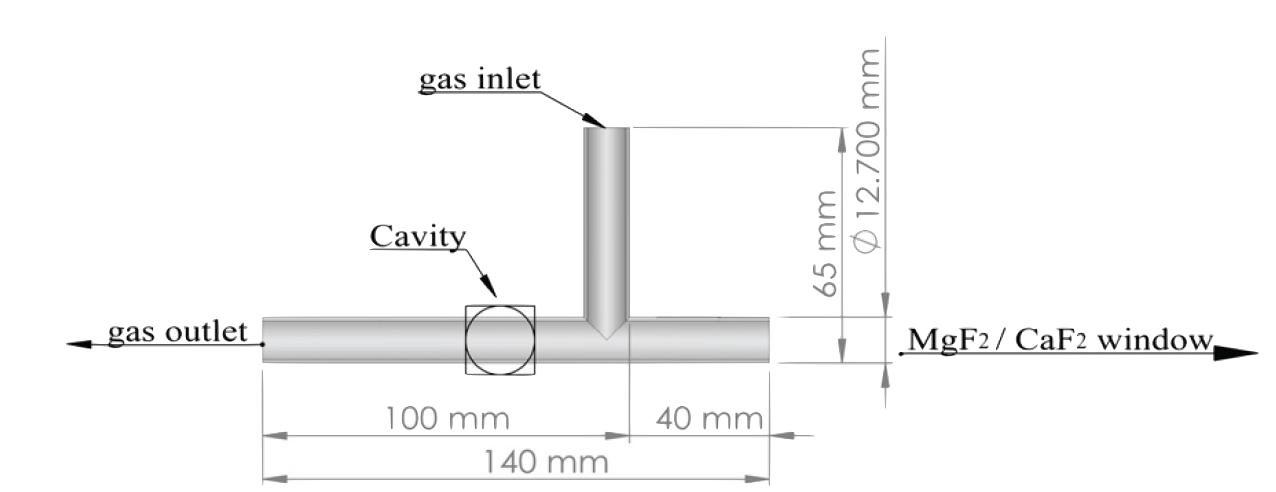
\includegraphics[width=\textwidth]{figures/chapter2/T_type.png}
\caption{The cross-section of MDHL (T-type geometry) (Quoted from Chen et al. 2014).}
\label{fig:T_type}
\end{figure}
In order to measure the photon flux in situ, we use an 88 \% transmittance nickel mesh with its photoelectric efficiency being obtained by high-flux beamline in National Synchrotron and a SXUV 100 photodiode calibrated by NIST. A MgF$_2$ window is placed between the lamp and the sample holder to prevent penetration of higher order VUV photons (with wavelength shorter than 114 nm). Figure \ref{fig:MDHL} shows a VUV emission spectrum of a MDHL with a cut off at 114 nm.
\begin{figure}
\centering
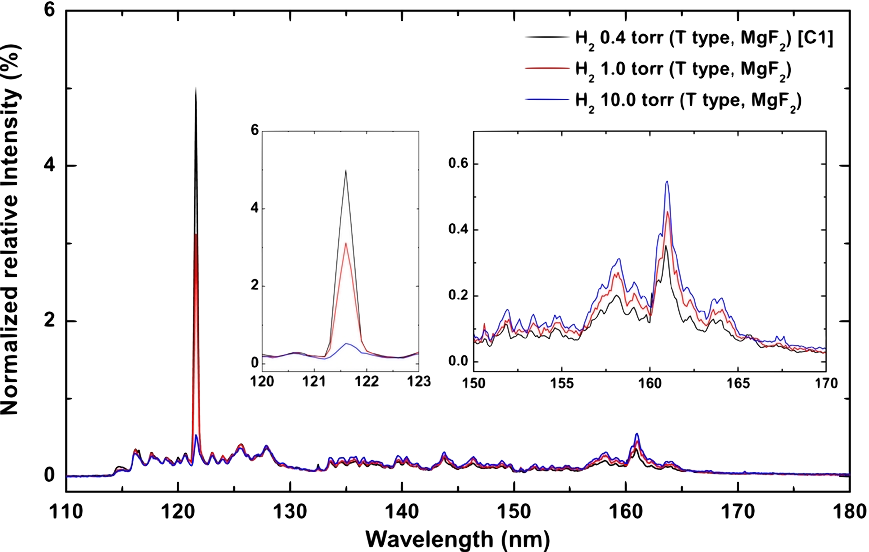
\includegraphics[width=\textwidth]{figures/chapter2/MDHL.png}
\caption{VUV spectra of MDHL (T-type geometry, 110-180 nm) with different H$_2$ pressure inside the lamp(Quoted from Chen et al. (2014)\cite{chen2013vacuum}) .}
\label{fig:MDHL}
\end{figure}
It consists of Ly-α (121.6nm) photons and H$_2$ molecular emission in the range of 110-180 nm. Chen et al. (2014) showed that the spectral characteristics of the VUV light emitted in this range depends on the gas type (mixture of H$_2$ with He or Ar etc), pressure of H$_2$ and lamp geometry \cite{chen2013vacuum}. Throughout those configurations stated there, we adopted 0.4 torr molecular hydrogen and T-type MDHL that produces VUV irradiation at 114-170 nm with 19.1 \% of Ly-α photons and a mean photon energy of 9.27 eV. The photon flux is $6.4 \times 10^{13}$ photons $cm^{-2} s^{-1}$ at sample position.

\subsection{Extreme EUV source}
\label{sec:Extreme_EUV_source}

To simulate the solar EUV irradiation on both Charon and interstellar ices, we use the HF-CGM high – flux beam line of the National Synchrotron Radiation Research Center in Hsinchu, Taiwan. It provides a continuum EUV to VUV photons from 4 to 40 eV. The continuum is separated into monochromatic 30.4nm (40.8 eV)photons with a six-meter cylindrical grating monochrometer with an incident angle of 70 degrees. With the help of a movable entrance slit and movable curved exit slit, the energy resolving power can reach around $3 \times 10^4$ at 40 eV for grating 1600 l/mm with both slits movable and set opening to 10 $\mu m$ \cite{hsieh1998design}. Similar to VUV irradiation provided by MDHL, the light intensity is monitored by the same nickel mesh with photoelectric efficiency obtained by SXUV 100 photodiode calibrated by NIST. With the known photoelectric efficiency, the flux of monochromatic 30.4nm (40.8 eV) is measured to be $2.15 \times 10^{14}$ photons $s^{-1} cm^{-2}$, which is in the same order of magnitude of VUV continuum of MDHL. We replace the port with MDHL by the end station of the high-flux beamline. To prevent contaminations in the pipes and bellows, we place a cryostat backed up by a scroll pump between our system and the beamline endstation. Between the cryostat and our main chamber is a SiO$_2$ valve, which is sealed to prevent contamination to the end station during the warm-up phase.

\section{Experimental Protocol}
\label{sec:Experimental_Protocol}

In this section, we will briefly introduce the  procedures of how we perform our experiments. It is divided into four parts, preparation and cooling, deposition, irradiation and warmup.

\subsection{Preparation of experiments and cooling}
Before any of experiment is done, we bake our system at $100 \,^{\circ}\mathrm{C}$, for 48 hours to reduce the contamination of water and residue gases as much as possible. It is cooled to room temperature that the background pressure can reach routinely at $~ 1 \times 10^{-10}$ torr. The gasline is connected with the regulators of the gas tanks and bake to $100\,^{\circ}\mathrm{C}$ and pumped by turbomolecular pump for two days before any experiments are done. Before cooling the substrate to cryogenic temperature, we take an infrared(IR) spectrum and start the monitoring of residue gases by QMS in order to compare the residue molecules and to verify any possible contaminations in the main chamber. We then start the cooling process with the help of the closed-cycle He cryostat.

\subsection{Deposition}
The gas mixtures are pre-mixed in our gasline system introduced in section \ref{sec:IPS_system}. We control the relative proportion of two ice mixtures by sealing corresponding partial pressure gases in two equal volumn stainless steel bottles. We condense the gas premixed in the stainless steel bottles onto pre-cooled KBr substrate via leak valve. The substrate is monitored by Fourier-Transform Infrared (FTIR) Spectrometer and Quadrupole mass spectrometer (QMS) during deposition. The pressure of deposition is fixed to $1 \times 10^{-8}$ torr that the deposition rate is around 4 $\times$ 10$^{16}$ molecules cm$^{-2}$ min$^{-1}$, which varies in different relative ratio of our ice mixtures because the differences in sticking coefficients. After deposition, we place the ice mixture at 15 K for 60 minutes and allow pumping of residue gases, until the pressure of the main chamber falls back to its base pressure to simulate the interstellar environment before any irradiation.

\subsection{Photon Irradiation}
The total irradiation time is 270 minutes (with some 450 minutes, depend on experiment configurations) with time intervals varies from 2 to 30 minutes. After each irradiation, we wait for 10 minutes allowing pumping out of the photodesorbed gas molecules. During irradiation, the photon flux is monitored by a nickel mesh. After Irradiation, we place the sample for 30 minutes in case if any further reaction is processed.

\subsection{Warmup}
We heat the tip of cold finger to 300 K (measured by silicon diode near the substrate) with rate 1 K/min. During warmup, we record the QMS from 1 to 100 a.m.u. to observe if there are low quantity of higher mass products formed during irradiation. Apart from QMS, we scan infrared spectra with 5 K intervals to monitor the evolution of infra-red active species such as photo products and reactants. With both infra-red and QMS, we may better identify the photo products by kinetic energy gained during warm-up and temperatures the desorpted.

\section{Infra-red spectroscopy and the Beer-Lambert’s Law}
\label{sec:spectroscopy}
We use infra-red spectroscopy extensively in chapter \ref{results}. It is a powerful tool to study molecular interactions during irradiation and warmup. We choose infra-red rather than Raman spectroscopy because infra-red has lower energy that it would not change the structure of the ice mixture nor breaking any of the bonds. In addition, it is also much richer in terms of identifying functional groups especially when studying ice mixtures whose vibrational modes falls in the mid-IR wavelength ranges. With different vibrational modes, the energy absorbed by molecules are quantified. With the energy of absorption bands in infra-red spectrum, we may identify the functional group of the species. To simply classify, vibrational motions can be divided into stretching and bending. Stretching needs more energy than bending. For stretching, there are symmetric and asymmetric stretchings; while bending can be divided into in-plane (scissoring, rocking) and out-of-plane (wagging and twisting) (Figure \ref{fig:vibration}).
\begin{figure}
\centering
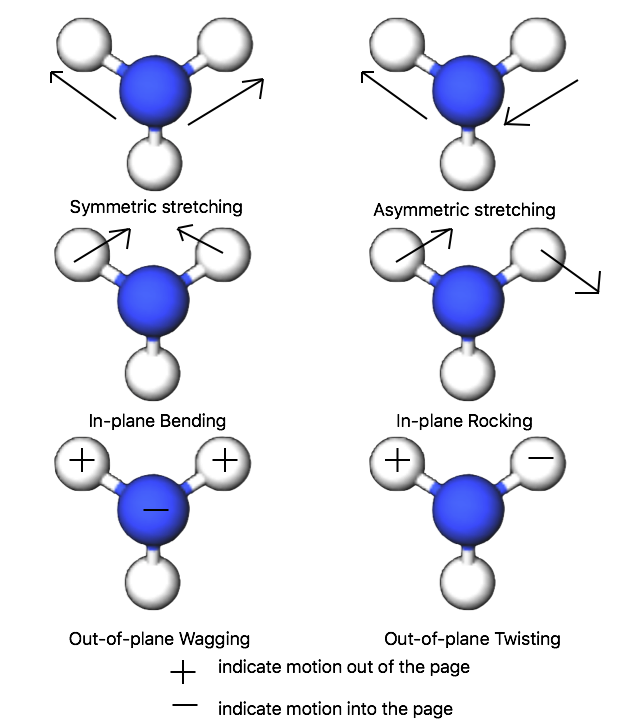
\includegraphics[width=\textwidth]{figures/chapter2/vibration.png}
\caption{Different vibrational modes of a three atom molecule.}
\label{fig:vibration}
\end{figure}

By Beer’s Law, we may calculate the column density of the molecule with its functional groups, which are used to plot figures in chapter 3 and 4. Beer Lambert’s Law suggests that when light passes through a medium, the amount of light absorbed is proportional to density and path length of the medium. Assume a known intensity beam $I_{0}(\nu)$ passes through the medium and beam intensity become $I(\nu)$. The transmittance $T(\nu)$ is defined by equation \ref{eq:transmittance}. \\
\begin{equation}
T(\nu) = \frac{I(\nu)}{I_{0}(\nu)}
\label{eq:transmittance}
\end{equation}
Also, the absorbance $a(\nu)$ is defined by equation \ref{eq:absorbance}. \\
\begin{equation}
a(\nu) = - \ln T(\nu) = - \ln \frac{I(\nu)}{I_{0}(\nu)} = n l \sigma(\nu)
\label{eq:absorbance}
\end{equation}
where $n$ is number density (molecules/cm$^3$), $l$ is the path length (cm), $\sigma(\nu)$ is the cross-section (cm$^2$/molecule) of corresponding frequency $\nu$. This equation is known as Lambert Beer’s Law. \\

As the ice mixtures in our thesis are at 15 K, the peaks of absorbance are often a broadband due to coupling between neighbor molecules. Therefore, we can integrate the whole band of the peak by equation \ref{eq:absorbance} with respect to frequency. Combines the (integrated) absorbance band strength (A value) in literatures to calculate the column densities $N$ of the ices by equation \ref{eq:column_density}.

\begin{equation}
N = \frac{\int a(\nu) \mathrm{d}\nu}{A(\nu)}
\label{eq:column_density}
\end{equation}
where $N$ is the column density (molecule cm$^{-2}$), $A(\nu)$ is the absorbance strength (cm molecule$^{-1}$).

\section{Reaction Rate Laws}
\label{sec:Reaction_Rate_Laws}
In this section, we will introduce rate reaction of a consecutive reaction and the concept of pseudo first order which we use to fit our reaction product against photon dose in chapter \ref{results}. The rate of a chemical reaction is a change in concentration of a substance per unit of time.

To determine the order of a reaction, we can only determine it experimentally.
For a zero order reaction, the rate $ = - \frac{d[R]}{dt} = k[R]^0$. By calculus, $[R]_0 - [R]_t = kt$.

For a first order reaction, rate $ = - \frac{d[R]}{dt} = k[R]$. By calculus, $\ln [R]_t = -kt + \ln [R]_0$.

For a second order reaction, rate $ = - \frac{d[R]}{dt} = k[R]^2$. By calculus, $\frac{1}{[R]_t} - \frac{1}{[R]_0} = kt$.

In a reaction with one reactant in excess, the rate of reaction is called pseudo first order reaction where pseudo means pretended. For D+E $\rightarrow$ F, rate $ = k[D][E]$. As $[E]_0 \gg [D]_0$, change of $[E]$ is negligible that $[E] \sim [E]_0$. Therefore, $[E]$ is assumed to be a constant and included in the rate constant k.

For a consecutive reaction equation, which we used to fit our data points, where D $\rightarrow$ E $\rightarrow$ F that the produced product will not convert back as reactant. A simple example is radioactive decay. At $t=0$, $[D]=[D]_0$, $[E]=0$, $[F]=0$ and at all times, $[D]+[E]+[F]=[D]_0$. The rate equations are as follows:
\begin{equation}
\frac{ d[D]}{dt} = - k_1 [D]
\label{eq:rate1}
\end{equation}

\begin{equation}
\frac{d[B]}{dt} = k_1 [D] - k_2 [E]
\label{eq:rate2}
\end{equation}

\begin{equation}
\frac{\Delta [F]}{\Delta t} = k_2 [E]
\label{eq:rate3}
\end{equation}
By equation \ref{eq:rate1}, we get
\begin{equation}
[D] = [D]_0 e^{-k_1 t}
\label{eq:rate4}
\end{equation}
By substituting equation \ref{eq:rate4} into equation \ref{eq:rate2}, we get

\begin{equation}
- \frac{\Delta [E]}{\Delta t} + k_2 [E] = k_1 [D]_0 e^{-k_1 t}
\label{eq:rate5}
\end{equation}
After solving the differential equation \ref{eq:rate5} , we get
\begin{equation}
[E] = \frac{k_1}{k_2 - k_1} (e^{-k_1 t} - e^{-k_2 t}) [D]_0
\label{eq:rate6}
\end{equation}
Finally, since $[F]=[D]_0 -[E]-[D]$, by equation \ref{eq:rate4} and \ref{eq:rate6}, we get
\begin{equation}
[F] = \Bigg( 1+ \frac{k_1 e^{-k_2 t} - k_2 e^{-k_1 t}}{k_2 - k_1} \Bigg) [D]_0
\label{eq:rate7}
\end{equation}
